% #############################################################################
% This is Chapter 5
% !TEX root = ../main.tex
% #############################################################################
% Change the Name of the Chapter i the following line
\fancychapter{Software Implementation and Simulation Results}
\cleardoublepage
% The following line allows to ref this chapter
\label{chap:results}


\section{Description of the Implemented Code}
\label{sec:description_implementation}

\par The variables for the motion planning problem are each vehicle's state variables and inputs, as explained in section \ref{sec:theoptproblem}. Each of these variables will be referred to as \textit{curves}. optimization algorithms cannot take continuous functions as variables, therefore, some form of parameterization of each curve is necessary, as exemplified in some of the algorithms of chapter \ref{chap:theory}. Here, each curve will be represented as a Bernstein Polynomial with order $N$, which will require $N+1$ control points. A distinction is made between state variables and inputs: state variables must have established initial and final conditions, inputs do not. This implies that for state variables, the initial and final control points must be fixed; therefore, they do not need to participate on the optimization problem. The following matrix represents how the control points are stored so that they can be accessed by all functions that perform operations on the curves.

\begin{equation}
    \begin{bmatrix}
        \colorbox{yellow}{$\displaystyle x_0^0$} & \colorbox{yellow}{$\displaystyle y_0^0$} & \colorbox{yellow}{$\displaystyle \psi_0^0$} & \colorbox{yellow}{$\displaystyle u_0^0$} & \colorbox{yellow}{$\displaystyle v_0^0$} & \colorbox{yellow}{$\displaystyle r_0^0$} & \tau_{u_0}^0 & \tau_{r_0}^0 \\
        x_1^0 & y_1^0 & \psi_1^0 & u_1^0 & v_1^0 & r_1^0 & \tau_{u_1}^0 & \tau_{r_1}^0 \\
        \vdots & \vdots & \vdots & \vdots & \vdots & \vdots & \vdots & \vdots \\
        \colorbox{yellow}{$x_{N}^0$} & \colorbox{yellow}{$y_{N}^0$} & \colorbox{yellow}{$\psi_{N}^0$} & \colorbox{yellow}{$u_{N}^0$} & \colorbox{yellow}{$v_{N}^0$} & \colorbox{yellow}{$r_{N}^0$} & \tau_{u_{N}}^0 & \tau_{r_{N}}^0
    \end{bmatrix}
    \label{eq:matrixofvariables}
\end{equation}

\par It is believed that \texttt{fmincon()} performs better when all variables are stored in a line vector \cite{privateconversationendpoints}; therefore, a function called \texttt{matrify()} is necessary in order to transform the flattened optimization variable to the matrix of equation (\ref{eq:matrixofvariables}). 
\par Elements marked in yellow do not participate in the optimization algorithm. They are concatenated to this matrix in \texttt{matrify()}. 

\par High orders are preferable for each curve \cite{cichella2018bernstein} because the higher the curve, the closer the control points are to the "matching" point in time of the curve, which is achieved once an optimization problem finishes. Chapter \ref{chap:results} shows how the control points approximate to the curve and how it is advantageous to produce the dynamics.


\par The optimization problem is formulated by constructing a data structure with the fields of table \ref{tab:constants_description}.


\begin{table}[]
\centering
\begin{tabular}{|l|l|l|l|}
\hline
\textbf{field} & \textbf{description} & \textbf{mandatory} & \textbf{example} \\ \hline
\texttt{T} & Time horizon & yes & \texttt{10} \\ \hline
\texttt{xi} & initial conditions & yes & \texttt{[0 0 0 1 0]} \\ \hline
\texttt{xf} & final conditions & yes & \texttt{[5 5 pi/2 1 0]} \\ \hline
\texttt{N} & order of the curves & yes & \texttt{15} \\ \hline
\texttt{obstacles} & polygons & \begin{tabular}[c]{@{}l@{}}no\\ default: \texttt{[]}\end{tabular} &  \\ \hline
\texttt{obstacles\_circles} & circles & \begin{tabular}[c]{@{}l@{}}no\\ default: \texttt{[]}\end{tabular} &  \\ \hline
\texttt{min\_dist\_int\_veh} & \begin{tabular}[c]{@{}l@{}}minimum distance between \\ vehicles for every point in time\end{tabular} & \begin{tabular}[c]{@{}l@{}}no\\ default: \texttt{0}\end{tabular} & \texttt{.8} \\ \hline
\texttt{numinputs} & \begin{tabular}[c]{@{}l@{}}number of input variables\\ (don't have initial conditions)\end{tabular} & \begin{tabular}[c]{@{}l@{}}no\\ default: \texttt{0}\end{tabular} &  \\ \hline
\texttt{uselogbar} & \begin{tabular}[c]{@{}l@{}}make the problem completely \\ unconstrained and use log \\ barrier functionals\end{tabular} & \begin{tabular}[c]{@{}l@{}}no\\ default: \texttt{false}\end{tabular} &  \\ \hline
\texttt{usesigma} & \begin{tabular}[c]{@{}l@{}}a boolean for the use of the \\ sigma function if log barrier \\ functionals are to be used\end{tabular} & \begin{tabular}[c]{@{}l@{}}no\\ default: \texttt{false}\end{tabular} &  \\ \hline
\texttt{costfun\_single} & \begin{tabular}[c]{@{}l@{}}a function used to calculate \\ the running cost for each \\ singular vehicle\end{tabular} & yes & \texttt{@costfun} \\ \hline
\texttt{dynamics} & \begin{tabular}[c]{@{}l@{}}a function that describes how the \\ non linear dynamics of the state \\ variables and inputs are linked\end{tabular} & yes & \texttt{@dynamics} \\ \hline
\texttt{init\_guess} & \begin{tabular}[c]{@{}l@{}}a function that provides an initial \\ guess for the optimization problem \\ which may  speed up the process \\ of optimization\end{tabular} & \begin{tabular}[c]{@{}l@{}}no \\ default:\\ \texttt{@rand\_init\_guess}\end{tabular} & \texttt{@init\_guess} \\ \hline
\texttt{recoverxy} & \begin{tabular}[c]{@{}l@{}}a function that returns the x and y\\ variables by solving just the initial \\ value problem of the inputs\end{tabular} & yes & \texttt{@recoverxy} \\ \hline
\end{tabular}
\caption{Description of the constants for optimization}
\label{tab:constants_description}
\end{table}


\par Some notes for each of the fields:

\begin{itemize}
    \item \texttt{xi} has as many lines as state variables (not input variables) and as many lines as number of vehicles. Because these functions are designed for vehicles, $x$ and $y$ must be in the first 2 columns
    \item \texttt{xf} works just as \texttt{xi}
    \item \texttt{obstacles\_circles}  Ncircles by 3, where columns are x, y and radius, respectively
    \item \texttt{recoverxy} takes an aribtrary $X$ matrix and and a \texttt{constants} structure and returns a Npoints by 2 matrix
    \item \texttt{dynamics} takes in an arbitrary X matrix and constants structure (to provide pre computer information like a derivation matrix) and must return a column vector which is zeros when all of the dynamic constraints are respected
\end{itemize}

\par The data structure for the nonlinear optimization problem is then passed to a function called \texttt{run\_problem} which returns the control points for each of the defined variable along with computation time.

\subsection{Dynamics}
\label{sec:dynamics}

\par The dynamics are guaranteed with the formulation of \ref{eq:multi_cost_bern}. This means that the code version for the dynamics plus kinematics for the Medusa vehicle, for example, which are  \ref{eq:simple_medusa_kinematics} and \ref{eq:simple_medusa_dynamics}, become

\begin{lstlisting}[language=matlabfloz,caption={\mcode{Dynamics Equality Constraint}}]
ceq = [
    DiffMat*x - u.*cos(yaw) + v.*sin(yaw) - Vcx;
    DiffMat*y - u.*sin(yaw) - v.*cos(yaw) - Vcy;
    DiffMat*yaw - r;
    DiffMat*u - 1/m_u*(tau_u + m_v*v.*r - d_u.*u+fu);
    DiffMat*v - 1/m_v*(-m_u*u.*r - d_v.*v+fv);
    DiffMat*r - 1/m_r*(tau_r + m_uv*u.*v - d_r.*r+fr);
];
\end{lstlisting}

\par As explained in section \ref{sec:theoptproblem}, \texttt{Diffmat} preserves the order and the equality is maintained in the control points, not the values of the curve itself so some approximation error is expected, which can be minimized with higher orders.

\par Given that each variable is defined by a set of control points, and, using the convex hull property of Bernstein polynomials, upper and lower bounds for each variable, state or input, become the biggest or smallest control point, respectively.


\section{Results}
\par The following results are based on solving the optimization problem \eqref{eq:multi_cost_bern} with the implementation described in chapter \ref{chap:implementation}. Simulations were carried out using Sequential Quadratic Programming \cite{10.1007/978-0-387-35514-6_7} on models presented in chapter \ref{chap:autonomousvehiclemodels}. Simulations were run on a 4 × Intel\textsuperscript{\textcopyright} Core\texttrademark i5-7200U CPU @ 2.50GHz processor. 
\par The unicycle model has a total of 5 state variables while the Medusa model has a total of 6 state variables plus 2 inputs. Upper and lower bounds for each variable for each vehicle were implemented, as explained in section \ref{sec:dynamics}, by finding the biggest and smallest control points of each polynomial. For the examples presented in this chapter, the bounds that were used are those presented in table \ref{tab:variablebounds} which were chosen to represent realistic values of a vehicle.

\begin{table}[h!]
\centering
\begin{tabular}{|l|l|l|l|}
\hline
& Variable & Lower Bounds & Upper Bounds \\ \hline
Dubin's Car & $x\ (\si{\meter})$ & $-\infty$ & $\infty$ \\
& $y\ (\si{\meter})$ & $-\infty$ & $\infty$ \\
& $\psi\ (\si{\radian})$ & $-\infty$ & $\infty$ \\
& $u\ (\si{\meter\per\second})$ & 0 & 1.1 \\
& $r\ (\si{\radian\per\second})$ & $-\pi/4$ & $\pi/4$ \\ \hline
Medusa & $x\ (\si{\meter})$ & $-\infty$ & $\infty$ \\
& $y\ (\si{\meter})$ & $-\infty$ & $\infty$ \\
& $\psi\ (\si{\radian})$ & $-\infty$ & $\infty$ \\
& $u\ (\si{\meter\per\second})$ & 0 & 1.1 \\
& $v\ (\si{\meter\per\second})$ & $-\infty$ & $\infty$ \\
& $r\ (\si{\radian\per\second})$ & $-.74$ & $.74$ \\
& $\tau_u\ (\si{\newton})$ & 0 & 25.9 \\
& $\tau_r\ (\si{\newton\meter})$ & -.113 & .113 \\
\hline
\end{tabular}
\caption{Upper and lower bounds for each variable of each vehicle model}
\label{tab:variablebounds}
\end{table}

\par A range of experiments were performed with the optimization algorithm in order to study its behaviour with changing parameters. Out of all of the experiments that were performed, the most relevant are presented here.


\subsection{No Obstacles}

\par The first problem considered here is, for both a single Dubin's car and a single Medusa vehicle, with initial and final states described in table \ref{tab:firstproblem} and with no obstacles. Figure \ref{fig:noobstaclesfigures} show solutions for order 20 and a time horizon of \SI{60}{\second}. The top two plots minimize the square of the surge of the Dubin's car and Medusa vehicle, while the bottom two minimize the thrust $\tau_u$ and torque $\tau_r$, respectively. This figure, and all other figures, flip x and y axis which is standard for marine vehicles.

\begin{table}[h!]
\centering
\begin{tabular}{|l|l|l|}
\hline
Variable & Starting Conditions & Final Conditions \\ \hline
$x\ (\si{\meter})$ & 0 & 30 \\
$y\ (\si{\meter})$ & 0 & 30 \\
$\psi\ (\si{\radian})$ & 0 & $\pi/2$ \\
$u\ (\si{\meter\per\second})$ & 1 & 1 \\
$v\ (\si{\meter\per\second})$ & 0 & 0 \\
$r\ (\si{\radian\per\second})$ & 0 & 0 \\
\hline
\end{tabular}
\caption{Initial and final conditions for a basic Motion Planning Problem}
\label{tab:firstproblem}
\end{table}

\begin{figure}[h!]
\centering
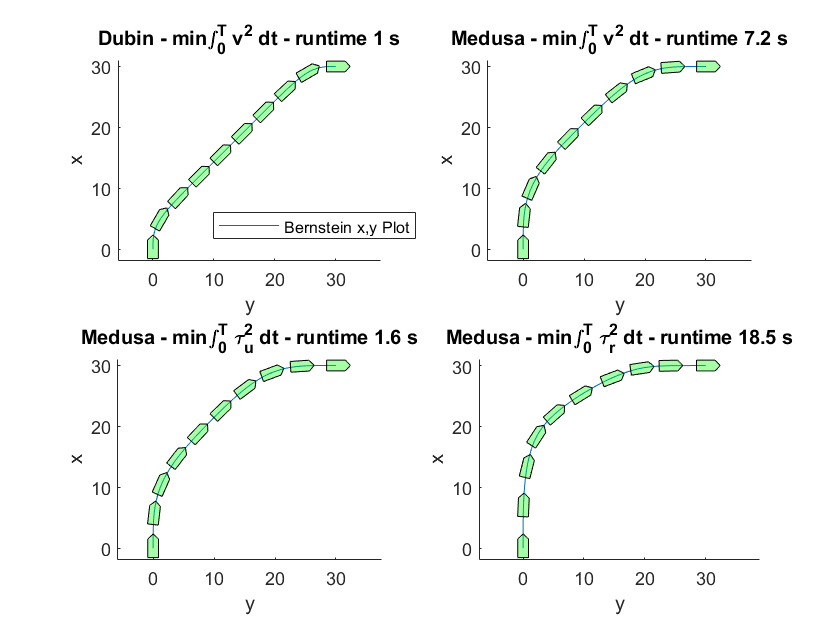
\includegraphics[width=\textwidth]{Images/results/noostaclesfigures.png}
\caption{Solutions of order $N=20$ without obstacles and final time $T=60$}
\label{fig:noobstaclesfigures}
\end{figure}

\par The ten plotted arrows in each plot show the position and heading of the vehicles over equidistant time intervals. The closer the arrows are to each other, the slower the vehicle are during the respective time interval. The initial guess that is provided to these examples are a set of random values that respect the variable bounds established earlier. These examples serve as baselines for comparison once obstacles and multiple vehicles are introduced in the next sections.


\subsection{Obstacles}

\par Obstacle avoidance is implemented with the algorithms explained in sections \ref{sec:mindistintveh} and \ref{sec:mindistconvshapes}. The top left solution of figure \ref{fig:noobstaclesfigures} serves as the baseline for comparison without obstacles. Specifically, the solutions presented in this section use the same velocity minimisation running cost (min $\int_0^T v^2$), the same initial and final conditions (\ref{tab:firstproblem}), and the same order of polynomial $N=20$ for the Dubin's car. The only difference is the presence of the different obstacles. Figure \ref{fig:obstaclesfigures} show the solutions of the performed tests. The titles of the plots which say "Constrained" refer to when the environmental obstacle is implemented as an optimization constraint. The titles which say "Unconstrained" refer to plots resulting from unconstrained optimization, i.e., the environmental constraint was moved to the cost via the Log Barrier Functional. It is expected that the trajectories of the unconstrained problems are not perfectly tangent to the circle. If the running cost were not added to the total cost, the trajectory would be as far away as possible from the curve while still respecting the dynamic constraints; this is because the derivative of the Log Barrier Functional is always lower than zero even when the solution is feasible. The gap that we see between the curve and the obstacle is the result of balancing the running cost and the Log Barrier component. One implication is that running cost can never be ideal because the vehicle had to travel an extra amount of distance. Using the Log Barrier function, however, has the advantage of potentially reducing the runtime of the optimization process, as can be seen by comparing the computation times of the problems with the polygon obstacles. Furthermore the large difference in computation time between polygon obstacles and circle obstacles can be explained by the fact that the \textit{Minimum Distance to Polygon} algorithm is iterative, which means that all of the duration of the individual runs quickly add up.


\begin{figure}[h!]
\centering
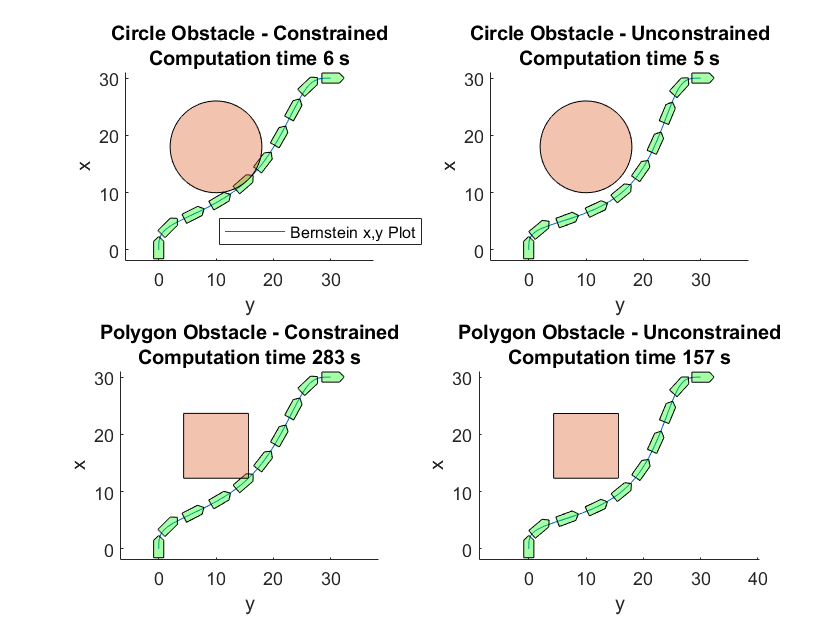
\includegraphics[width=\textwidth]{Images/results/ostaclesfigures.png}
\caption{Solution of order $N=20$ with obstacles and final time $T=60$}
\label{fig:obstaclesfigures}
\end{figure}


\subsection{Variation of cost with order}

\par A way of calculating solutions for high orders while maintaining low computation time is by running the optimization process on a random guess with low order, then perform degree elevation which increases the order of the solution and re-feed that solution to the same problem as the initial guess. In order to demonstrate this process, a new optimization problem was is presented. It uses the Dubin's car but with initial and final conditions given by table \ref{tab:increasingNproblem}. 

\begin{table}[h!]
\centering
\begin{tabular}{|l|l|l|}
\hline
Variable & Starting Conditions & Final Conditions \\ \hline
$x\ (\si{\meter})$ & 0 & 30 \\
$y\ (\si{\meter})$ & 0 & 30 \\
$\psi\ (\si{\radian})$ & $\pi/4$ & $\pi/4$ \\
$u\ (\si{\meter\per\second})$ & 1 & 1 \\
$r\ (\si{\radian\per\second})$ & 0 & 0 \\
\hline
\end{tabular}
\caption{Initial and final conditions for each step of the \textit{Increasing Order} Process}
\label{tab:increasingNproblem}
\end{table}


\par Figure \ref{fig:progressiveNexamples} shows the first, last, and two intermediary steps of this process. Figure \ref{fig:progressiveNinfo} shows the duration and cost of each intermediary run. The execution starts with order $N=10$, resulting the top left plot of the figure. This solution, then, has its order increased by 10, and is passed as an initial guess of the same problem but now with order 20.This process of increasing order stops when the final cost of the last run varies only by 1\% of previous run. For this particular example, the iterative process stops with order 70. The same problem of order 70 but with a random initial guess, took a total of 334 seconds, as opposed to 660 seconds, for the overall duration for all runs from order 10 to 70. Despite the total duration being nearly twice that for the run of order 70 with a random initial guess, this method may still be advantageous because the run of order 70 is faster, which suggests that with a good criterion for increasing order, the overall duration may be smaller. This method has the extra advantage of producing a solution we know is close to optimal. 



\begin{figure}[h!]
\centering
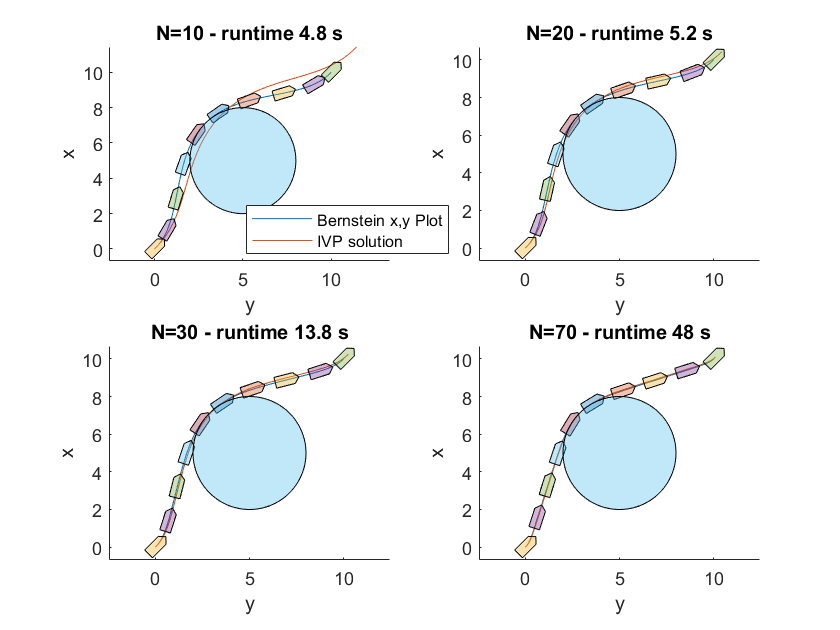
\includegraphics[width=\textwidth]{Images/results/progressiveNexamples.png}
\caption{Results of Interatively increasing order}
\label{fig:progressiveNexamples}
\end{figure}


\begin{figure}[h!]
\centering
\begin{subfigure}[b]{0.5\textwidth}
    \centering
    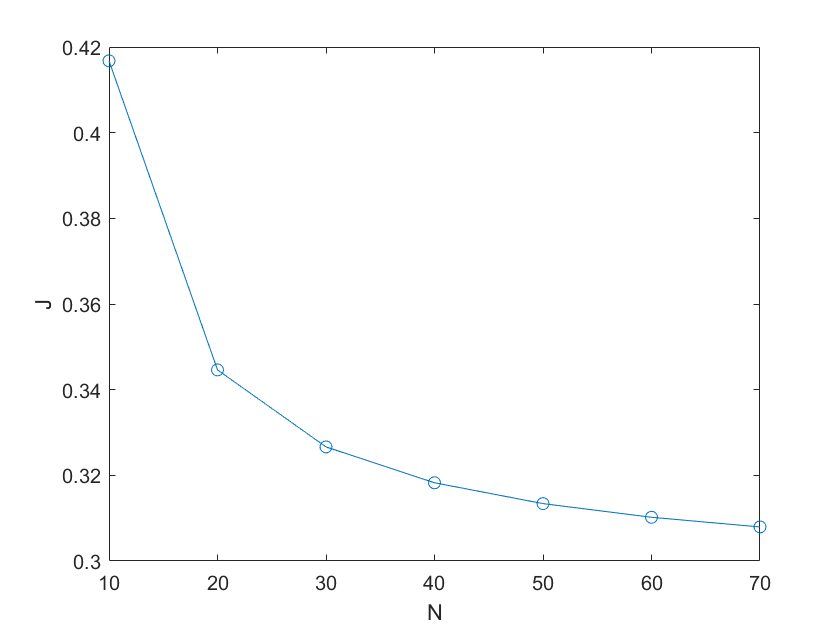
\includegraphics[width=\textwidth]{Images/results/costevolution.png}
    \caption{Evolution of Cost}
    \label{fig:evolutionofcostprogressiveN}
\end{subfigure}%
\begin{subfigure}[b]{0.5\textwidth}
    \centering
    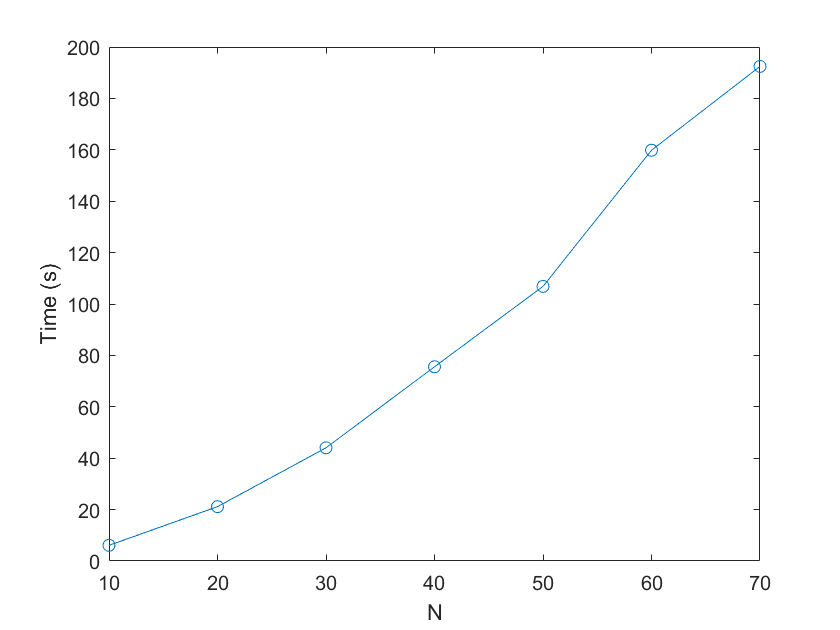
\includegraphics[width=\textwidth]{Images/results/timeevolutionincreasingN.png}
    \caption{Evolution of the final cost with each order}
    \label{fig:evolutionoftimeprogressiveN}
\end{subfigure}
\caption{Evolution of Cost and Time with Order Increase}
\label{fig:progressiveNinfo}
\end{figure}

\par Figure \ref{fig:ivpsoundness} shows, for order 10 on the left and order 70 on the right the two optimal solutions for the same problem, but this time, accompanied by the solution of the initial value problem, which integrates the speed and turn rate as explained in section \ref{sec:ivproblem}. With them, it can be seen how all of the variables returned by the motion planning algorithm are correctly linked with each other and how the higher the order, the more identical these curves are to one another.

\begin{figure}[h!]
\centering
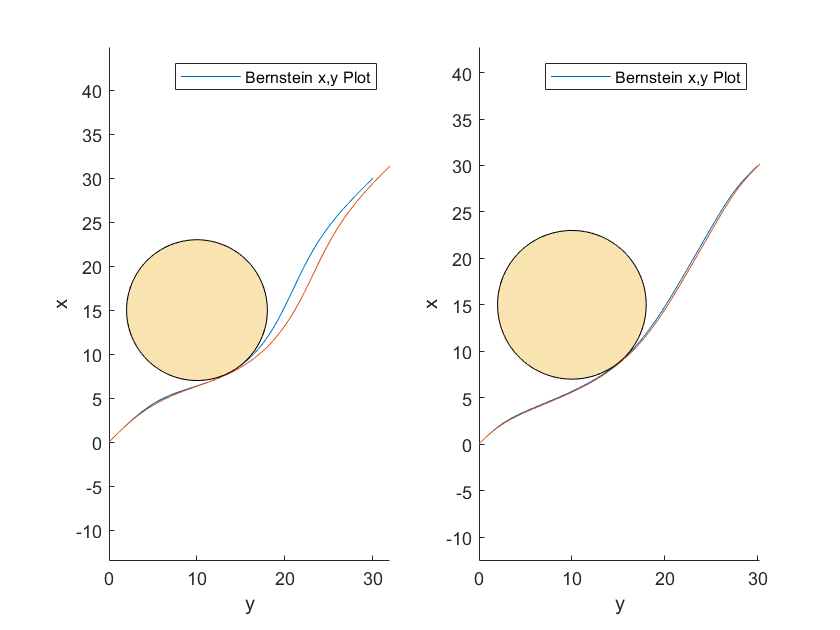
\includegraphics[width=\textwidth]{Images/results/ivpsoundness.png}
\caption{optimization solutions accompanied by the Initial Value Solutions}
\label{fig:ivpsoundness}
\end{figure}

\subsection{Multiple Vehicles}

\par To illustrate the use of multiple vehicles, a series of runs are presented in figure \ref{fig:multiplevehicles}. The initial and final conditions other than position are given by table \ref{tab:multivehconditions} with order $N=10$. Figure \ref{fig:timeevolutionmultiplevehicles} shows how the computation time increases with the added vehicles. These solutions are run with the inter vehicular constraints implemented as constraints on the optimization problem, as opposed to imposing them in the cost via the Log Barrier Functional. Specifically, the imposed constraint is a separation of \SI{3}{\meter} between trajectories calculated with the sampling based algorithm. Given that the problem focuses on trajectories, there is no problem in seeing the paths intersect. The same two vehicle problem with order $N=10$ takes a total of \SI{56}{\second} with the iterative \textit{Berstein to a point} algorithm which again shows how using an iterative algorithm with an optimization problems adds a lot of computation time.
\begin{table}[h!]
\centering
\begin{tabular}{|l|l|l|}
\hline
Variable & Starting Conditions & Final Conditions \\ \hline
$\psi\ (\si{\radian})$ & 0 & 0 \\
$u\ (\si{\meter\per\second})$ & 1 & 1 \\
$v\ (\si{\meter\per\second})$ & 0 & 0 \\
$r\ (\si{\radian\per\second})$ & 0 & 0 \\
\hline
\end{tabular}
\caption{Initial and final conditions for the Multiple Vehicles Problem}
\label{tab:multivehconditions}
\end{table}



\begin{figure}[h!]
\centering
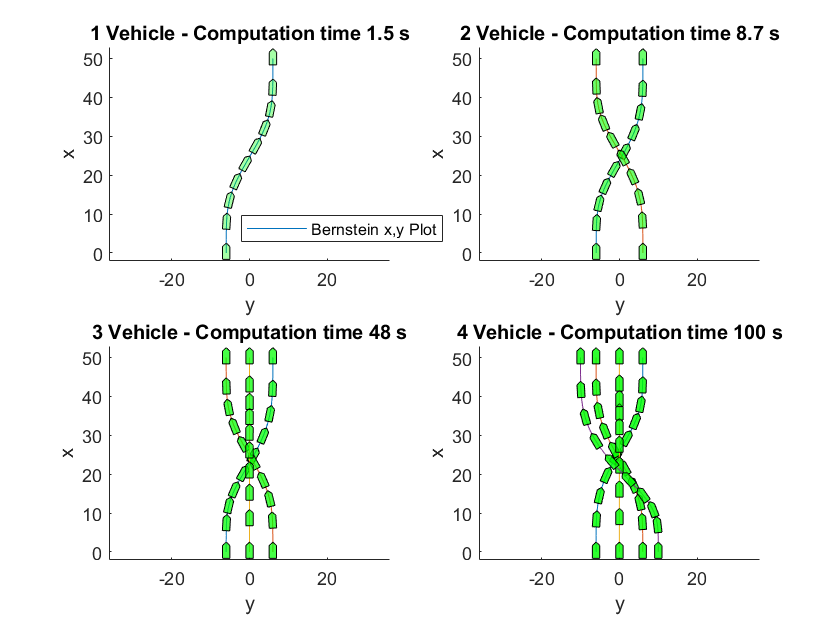
\includegraphics[width=\textwidth]{Images/results/multiplevehicles.png}
\caption{Solutions of order $N=10$ with multiple vehicles}
\label{fig:multiplevehicles}
\end{figure}

\begin{figure}[h!]
\centering
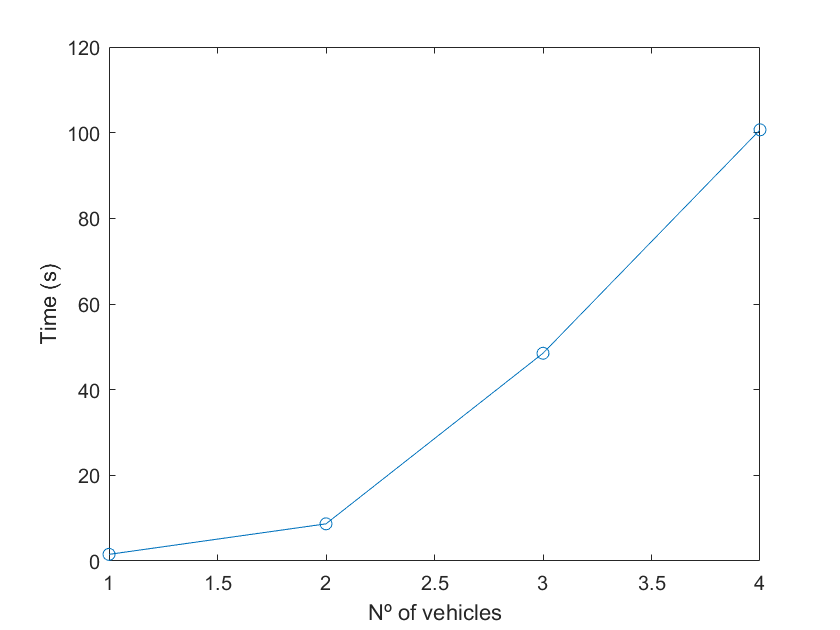
\includegraphics[width=0.8\textwidth]{Images/results/timeevolutionmultiplevehicles.png}
\caption{Evolution of Computation time with increasing number of vehicles}
\label{fig:timeevolutionmultiplevehicles}
\end{figure}


\subsection{Trajectory Tracking Soundness}

\par In section \ref{sec:ivproblem}, it was suggested that soundness of the solution can be verified by feeding the returned inputs into a trajectory tracking algorithm and calculating the resulting size of error correction term. The better the inputs, the lower is the needed correction. A trajectory tracking algorithm that can perform this task is not available here. This task is carried out based on a graphical comparison of the inputs returned by the motion planning algorithm and the inputs calculated by a conventional trajectory tracking algorithm, such as the one found in [21], which calculates the inputs solely on error to the desired position.
\par Figure \ref{fig:trajectrackedprob} shows the solution of a constrained optimization problem for the Medusa Vehicle with order $N=50$, with initial and final conditions given by table \ref{tab:soundnessproblem}. 

\begin{table}[h!]
\centering
\begin{tabular}{|l|l|l|}
\hline
Variable & Starting Conditions & Final Conditions \\ \hline
$x\ (\si{\meter})$ & 0 & 0 \\
$y\ (\si{\meter})$ & 0 & 40 \\
$\psi\ (\si{\radian})$ & 0 & $\pi/2$ \\
$u\ (\si{\meter\per\second})$ & 1 & 1 \\
$v\ (\si{\meter\per\second})$ & 0 & 0 \\
$r\ (\si{\radian\per\second})$ & 0 & 0 \\
\hline
\end{tabular}
\caption{Initial and final conditions for a Constrained Problem}
\label{tab:soundnessproblem}
\end{table}

\par The computation time of the optimization problem is \SI{113}{\second}. It also shows the result of applying the Trajectory Tracking controller in \cite{Vanni2007CoordinatedMC}. The inputs, which are surge and torque, are obtained by the optimization problem and the Trajectory Tracking algorithm are shown in figure \ref{fig:inputscomparison}. It can be seen that the resulting inputs look similar, which validates the solution of the optimization problem.

\begin{figure}[h!]
\centering
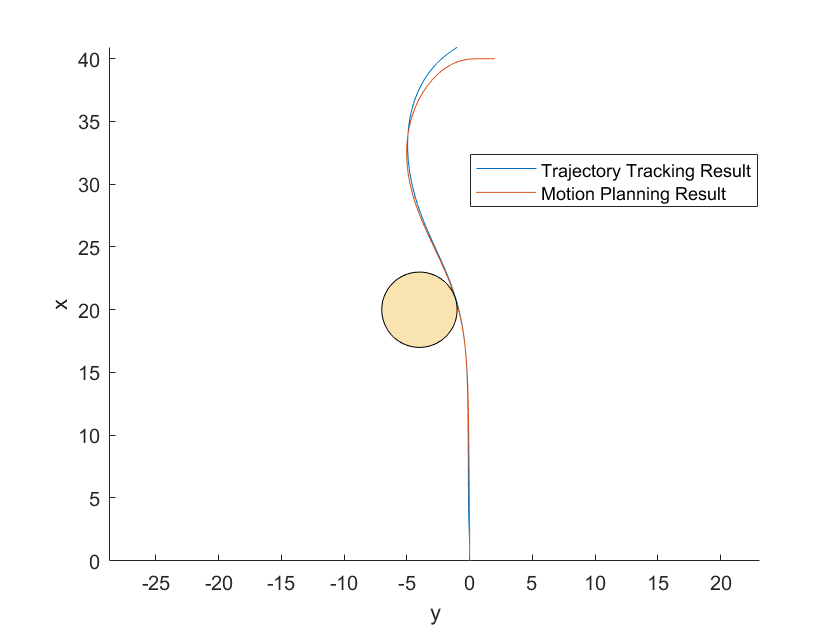
\includegraphics[width=0.8\textwidth]{Images/results/trajectrackedprob.png}
\caption{optimization Problem Solution and Trajectory Tracked Solution}
\label{fig:trajectrackedprob}
\end{figure}

\begin{figure}[h!]
\centering
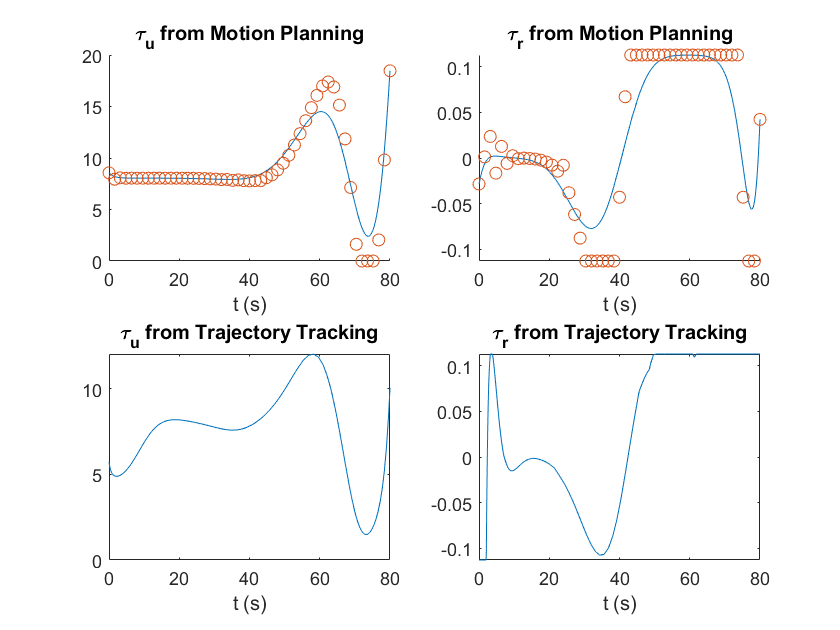
\includegraphics[width=0.8\textwidth]{Images/results/inputscomparison.png}
\caption{Comparison of the optimization Problem's Inputs and the Trajectory Tracking Inputs}
\label{fig:inputscomparison}
\end{figure}


\subsection{Final Example}
\par A final example of the application is shown in figure \ref{fig:finalexample}. It combines the various algorithms for inter-vehicle collision and obstacle avoidance  and the use of the Log Barrier Functional to achieve the fastest possible computation time.

\begin{figure}[h!]
\centering
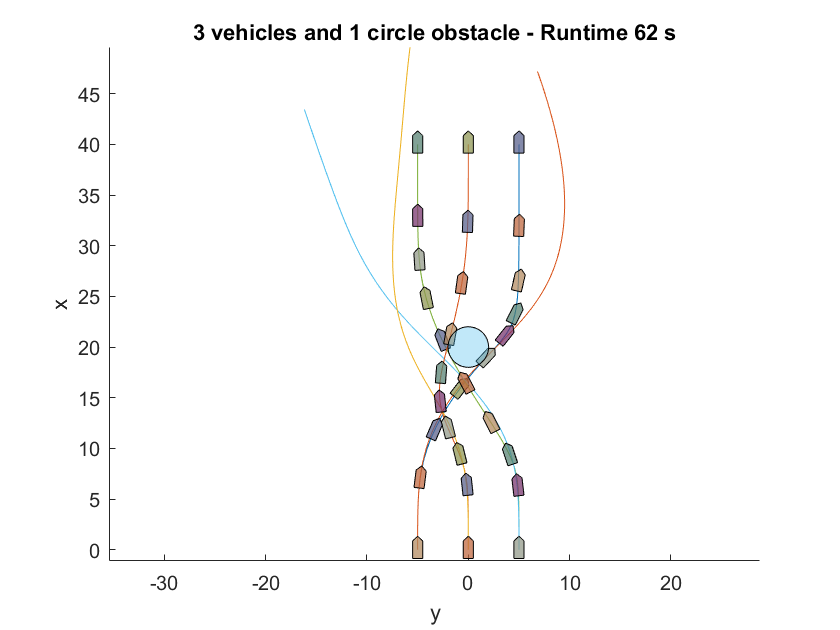
\includegraphics[width=\textwidth]{Images/results/finalexample.png}
\caption{Solution of order $N=10$ with 3 vehicles and 1 circle obstacle}
\label{fig:finalexample}
\end{figure}

